\maketitle
\setcounter{page}{1}
\tableofcontents
\newpage
\pagenumbering{arabic}
\section{Theorie}
Ziel des Versuchs ist die expermentelle Betrachtung des Röntgenemissionsspektrums
von Kupfer sowie verschiedener Absorbtionsspektren.
\subsection{Entstehung von Röntgenstrahlung}
Röntgenstrahlung entsteht bei der Wechselwirkung von beschleunigten Elektronen
mit Materie. Die Elektronen werden dabei in einer evakuiertien Röhre (der sogenannten
Röntgenröhre) unter Zuhilfenahme des glühelektrischen Effekts aus einer Kathode ausgelöst
und zu einer Anode hin beschleunigt. Beim Auftreffen auf das Anodenmaterial führen
zwei Prozesse zur Entstehung von Röntgenstrahlung:
\begin{itemize}
  \item [1.]\textbf{Bremsstrahlung:} Die Elektronen treten hierbei in Wechselwirkung mit den
  Coulombfeldern der Atomkerne des Anodenmaterials. Die durch den dabei folgenden
  Abbremsvorgang verloren gegangene Energie wird in Form eines Photons emittiert.
  Das resultierende Spektrum ist kontinuierlich. Es weist eine Grenzwellenlänge auf,
  unter der keine Röntgenstrahlung gemessen werden kann. Sie berechnet sich zu
  \begin{equation}
    \lambda_{\symup{min}} = \frac{hc}{e_0U}
  \end{equation}
  (mit $\textsc{Plankschem}$ Wirkungsquantum $h$, Vakuumlichtgeschwindigkeit $c$ und Elektronenruhemasse $e_0$)
  und entspricht der vollständigen Abbremsung des Elektrons, bei dem die
  aus der Beschleunigung gewonnene gesamte kinetische Energie umgewandelt wird.
  Dieses Spektrum ist kontinuierlich, es wird daher oft als kontinuierliches Bremsspektrum
  oder auch als Bremsberg bezeichnet.
  \item [2.] \textbf{Charakteristisches Spektrum} Das charakteristische Spektrum der Röntgenstrahlung
  resultiert aus der Ionisation der Anodenatome durch die einfallenden Elektronen.
  Die von der Kathode emittierten Elektronen schlagen dabei Elektronen aus den inneren
  Schalen der Atome. Elektronen aus höheren Schalen fallen in die entstandenen Löcher
  und emittieren dabei Röntgenquenten. Die Energie der Röntgenquanten entspricht dabei
  der Differenz zwischen dem Ursprungsniveau und dem Zielniveau des Elektrons. Aus der
  Beziehung
  \begin{equation}
    E_n = -E_{\symup{Ryd}} z_{\symup{eff}}^2 \cdot \frac{1}{n^2}
    \label{eqn:3}
  \end{equation}
  mit $\textsc{Rydberg}$-Energie $E_{\symup{Ryd}} \approx \SI{13.6}{\electronvolt}$
  lässt sich die Bindungsenergie einer Elektronenschale ermitteln.
  Die Konstante $z_{\symup{eff}} = z - \sigma$ gibt hierbei die effektive Kernladung
  berechnet aus der tatsächlichen Kernladung und der Abschirmkonstante $\sigma$ an.
  Die beim Abfall
  entstehenden scharfen Linien im Röntgenspektrum werden als $K_\alpha$, $K_\beta$,
  $L_\alpha$ etc. bezeichnet. Der Großbuchstabe gibt dabei an, auf welche Schale das
  Elektron fällt, der griechische Buchstabe wie viele Schalen darüber es sich ursprünglich
  befand.
  Da die Abschrimkonstante dabei für jedes Elektron der äußeren Schale unterschiedlich ist,
  unterscheiden sich auch die Bindungsenergien innerhalb der äußeren Schale.
  Dies führt dazu, dass eine Linie des charakteristischen Spektrums aus mehreren nah
  beieinanderliegenden Einzellinien besteht. Diese lassen sich mit eingem Aufwand auflösen,
  diese Linien werden als Feinstruktur bezeichnet. Diese Linien sind dem Bremsspektrum aufgesetzt
  siehe Abbildung \ref{abb:1}.
\end{itemize}
\subsection{Absorbtion von Röntgenstrahlung}
Bei der Wechselwirkung von Röntgenstrahlung unter \SI{1}{\mega\electronvolt} mit Materie
spielen im wesentlichen zwei Effekte eine Rolle. Zum einen die Comptonstreuung, die
nur in Absorbern mit wenigen Elektronen nennenswerte Auswirkungen hat und zum anderen
den inneren Photoeffekt. Die einstrahlenden Röntgenquanten treffen dabei auf die
Hüllenenelektronen der Absorberatome, wobei sie mit einer gewissen Wahrscheinlichkeit
absorbiert werden. Die Absorbtionswahrscheinlichkeit ist dabei antiproportional zur
Energie der einfallenden Röntgenstrahlung. Erreichen die Röntgenquanten jedoch die
Bindungsenergie der Elektronen einer Schale können sie diese ionisieren. Dabei steigt
die Absorptionsrate extrem an, es bildet sich eine sogenannte Absorptionskante die
mit dem Buchstaben der ionisierten Schale bezeichnet wird (siehe Abbildung \ref{abb:2}).
Auch hierbei muss die
Feinstruktur beachtet werden. Die Bindungsenergie eines Elektrons in einer Schale,
die diese Feinstruktur aufweist, berechnet sich dabei nach der $\textsc{Sommerfeldschen}$-
Feinstrukturformel
\begin{equation}
  E_{n,\, j} = -E_{\symup{Ryd}}  \left( z_{\symup{eff, \, 1}}^2 \cdot \frac{1}{n^2}
  + \alpha^2 z_{\symup{eff, \, 2}}^4 \cdot \frac{1}{n^3} \left( \frac{1}{j+1/2} -
  \frac{3}{4n} \right) \right)
\end{equation}
mit Hauptquentenzahl $n$, Gesamtdrehimpulsquantenzahl $j$ und Feinstrukturkonstante $\alpha$.
Die Bestimmung der Abschrimkonstante $\sigma$ aus dieser Beziehung ist jedoch extrem
kompliziert und kann auch aus der Energiedifferenz zwischen zwei Feinstrukturkanten
erfolgen.
\begin{figure}[h]
  \centering
  \subcaptionbox{Emmisionsspektrum\cite{prezi} \label{abb:1}}[0.49\textwidth]{
  \centering
    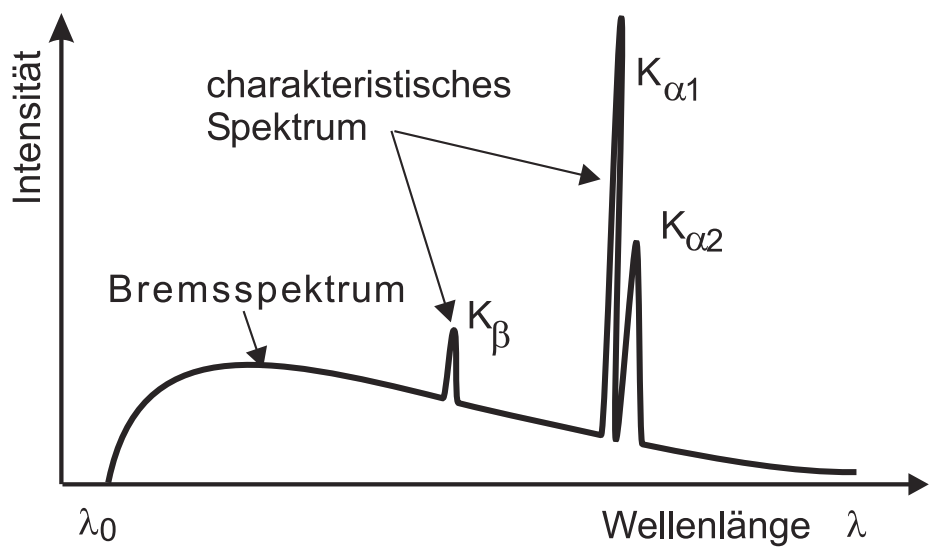
\includegraphics[width=0.49\textwidth]{Emissionsspektrum.png}
    }
  \subcaptionbox{Absorbtionsspektrum\cite{anleitung} \label{abb:2}}[0.49\textwidth]{
  \centering
    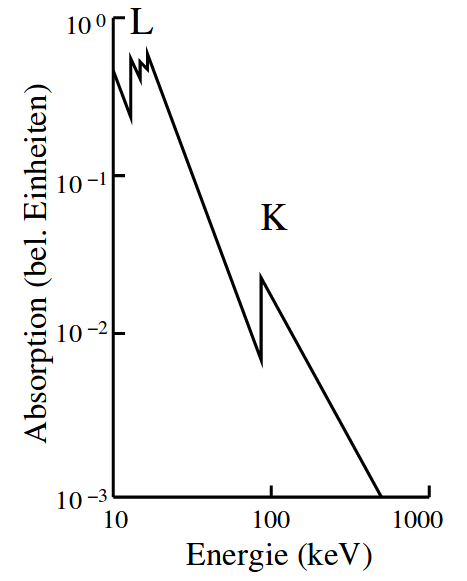
\includegraphics[width=0.3\textwidth]{Abs.png}
    }
  \hfill
  \caption{Emissions- und Absorbtionsspektrum von Röntengenstrahlung.}
\end{figure}
\subsection{Die Bragg-Gleichung}
Für Messungen an Röntgenstrahlung ist abschließend noch die $\textsc{Bragg}$-Gleichung
hilfreich. Die Röntgenquanten fallen dabei auf ein Gitter ein (beispielsweise ein
Einkristall) und werden dort in Abhängigkeit des Einfallswinkels gebeugt. Aus der Beziehung
\begin{equation}
  2 d \sin{\theta} = n \lambda
  \label{eq:3}
\end{equation}
folgt dann mit der Gitterkonstante $d$ zu jedem Winkel die Wellenlänge, die unter
diesem Winkel konstruktiv interferiert. $n$ gibt hierbei die Beugungsordnung an.
Dies ist in Abbildung \ref{abb:3} dargestellt.
\begin{figure}[h]
  \centering
  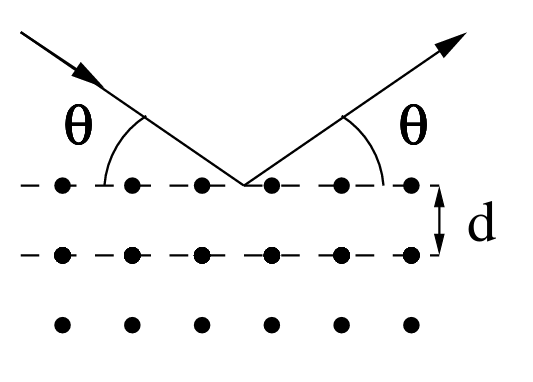
\includegraphics[scale=0.2]{braggtheo.png}
  \caption{Veranschaulichung der Beugung nach $\textsc{bragg}$ am Kristallgitter
  \cite{anleitung}.}
  \label{abb:3}
\end{figure}
\section{Durchführung}
\subsection{Versuchsaufbau}
Der Aufbau besteht aus einer Vorgefertigten Apperatur. In ihr befindet sich eine
Röntgenröhre mit Cu-Anode, ein drehbar gelagertes Geiger-Müller-Zählrohr sowie ein
LiF-Kristall. Auf dem Sensor des Geiger-Müller-Zählrohrs befindet
sich eine Blende, damit nur das erste Beugungsmaximum gemessen wird. Die Apperatur ist
mit einem Computer verbunden, an dem ein Programm die Messung automatisiert durchführen
kann. An der Röntgenröhre sind Beschleunigungsspannung und Emissionsstrom einstellbar.
Der Versuchsaufbau findet sich in Abbildung \ref{abb:4}.
\begin{figure}[h]
  \centering
  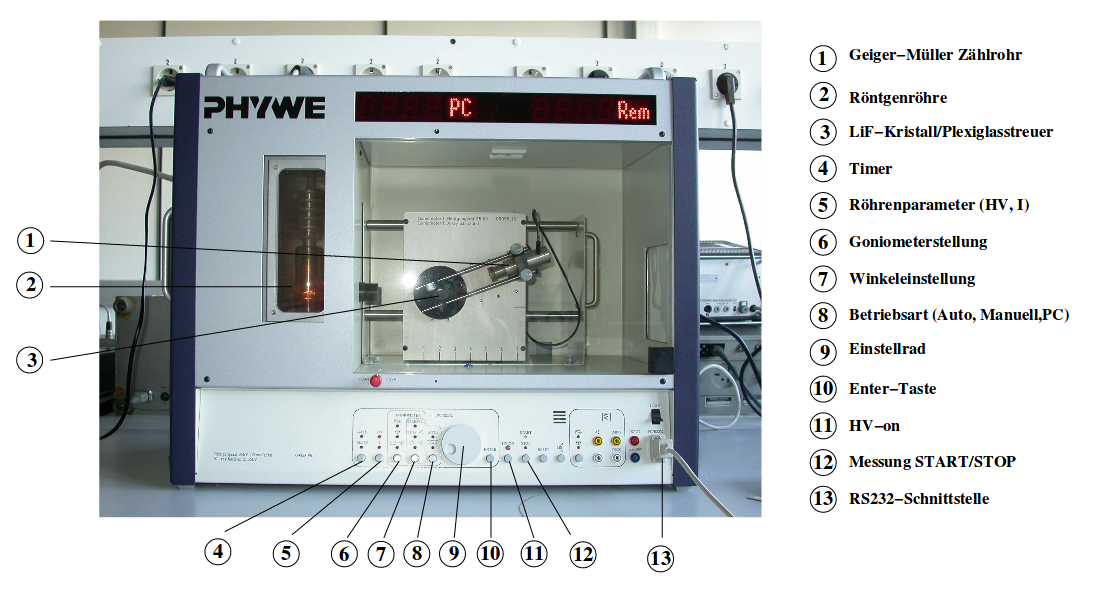
\includegraphics[scale=0.3]{Aufbau.png}
  \caption{Versuchsaufbau \cite{anleitung}.}
  \label{abb:4}
\end{figure}
\subsection{Versuchsdurchführung}
Der Versuch besteht aus drei Teilen:
\begin{enumerate}
  \item In einem ersten Versuchsteil wird die $\textsc{Bragg}$-Bedingung untersucht. Der Winkel
  des LiF-Kristalls wird dabei fest auf einen Winkel von \SI{14}{\degree}
  eingestellt und ein Winkelbereich von \num{26}
  bis \SI{30}{\degree} in \SI{0.1}{\degree}-Schritten mit
  dem Geiger-Müller-Zählrohr abgefahren. Das dabei bestimmte Maximum wird mit dem
  aus \eqref{eq:3} bestimmten Theoriewert verglichen.
  \item Im zweiten Versuchsteil wird im 2:1 Koppelmodus der Kristall von \num{4}
  bis \SI{26}{\degree} umfahren und in \SI{0.2}{\degree} Schritten für
  mindestens \SI{5}{\second} die Intensität
  gemessen. Mit der Bragg-Bedingung lässt sich hieraus das Emissionsspektrum der
  Röntgenröhre ermitteln.
  \item Im letzten Versuchsteil werden für \num{6} verschiedene Absorbermaterialen
  die Absorbtionsspektren aufgenommen. Die Absorber werden dabei vor dem Geiger-Müller-Zählrohr
  eingespannt und der Kristall in \SI{0.1}{\degree}-Schritten umfahren. Für jeden
  Winkel wird dabei ca. \SI{20}{\second} die Intensität gemessen. Aus den Messwerten
  lassen sich die Absorbtionsspektren bestimmen.
\end{enumerate}
\section{Auswertung}
\subsection{Überprüfen der Bragg-Bedingung}
In Abbildung \ref{fig:1} ist der Graph zur Überprüfung der Bragg-Bedingung zu finden.
Das Maximum liegt bei $\alpha_{GM} = 28.5°$. Der Sollwinkel liegt bei 28°, somit ist
die Bragg-Bedingung erfüllt.
\begin{figure}
  \centering
  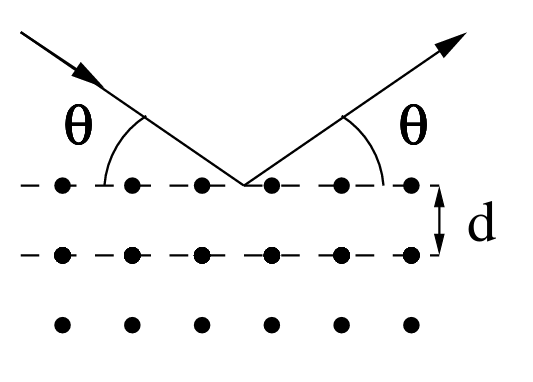
\includegraphics[scale=0.2]{bragg.png}
  \caption{Messung zur Überprüfung der Bragg-Bedingung.}
  \label{fig:1}
\end{figure}

\subsection{Emissionspektrum für Kupfer}
\begin{figure}
  \centering
  \subcaptionbox{Graphische Darstellung des Emissionspektrums. \label{fig:2}}[0.4\textwidth]{
  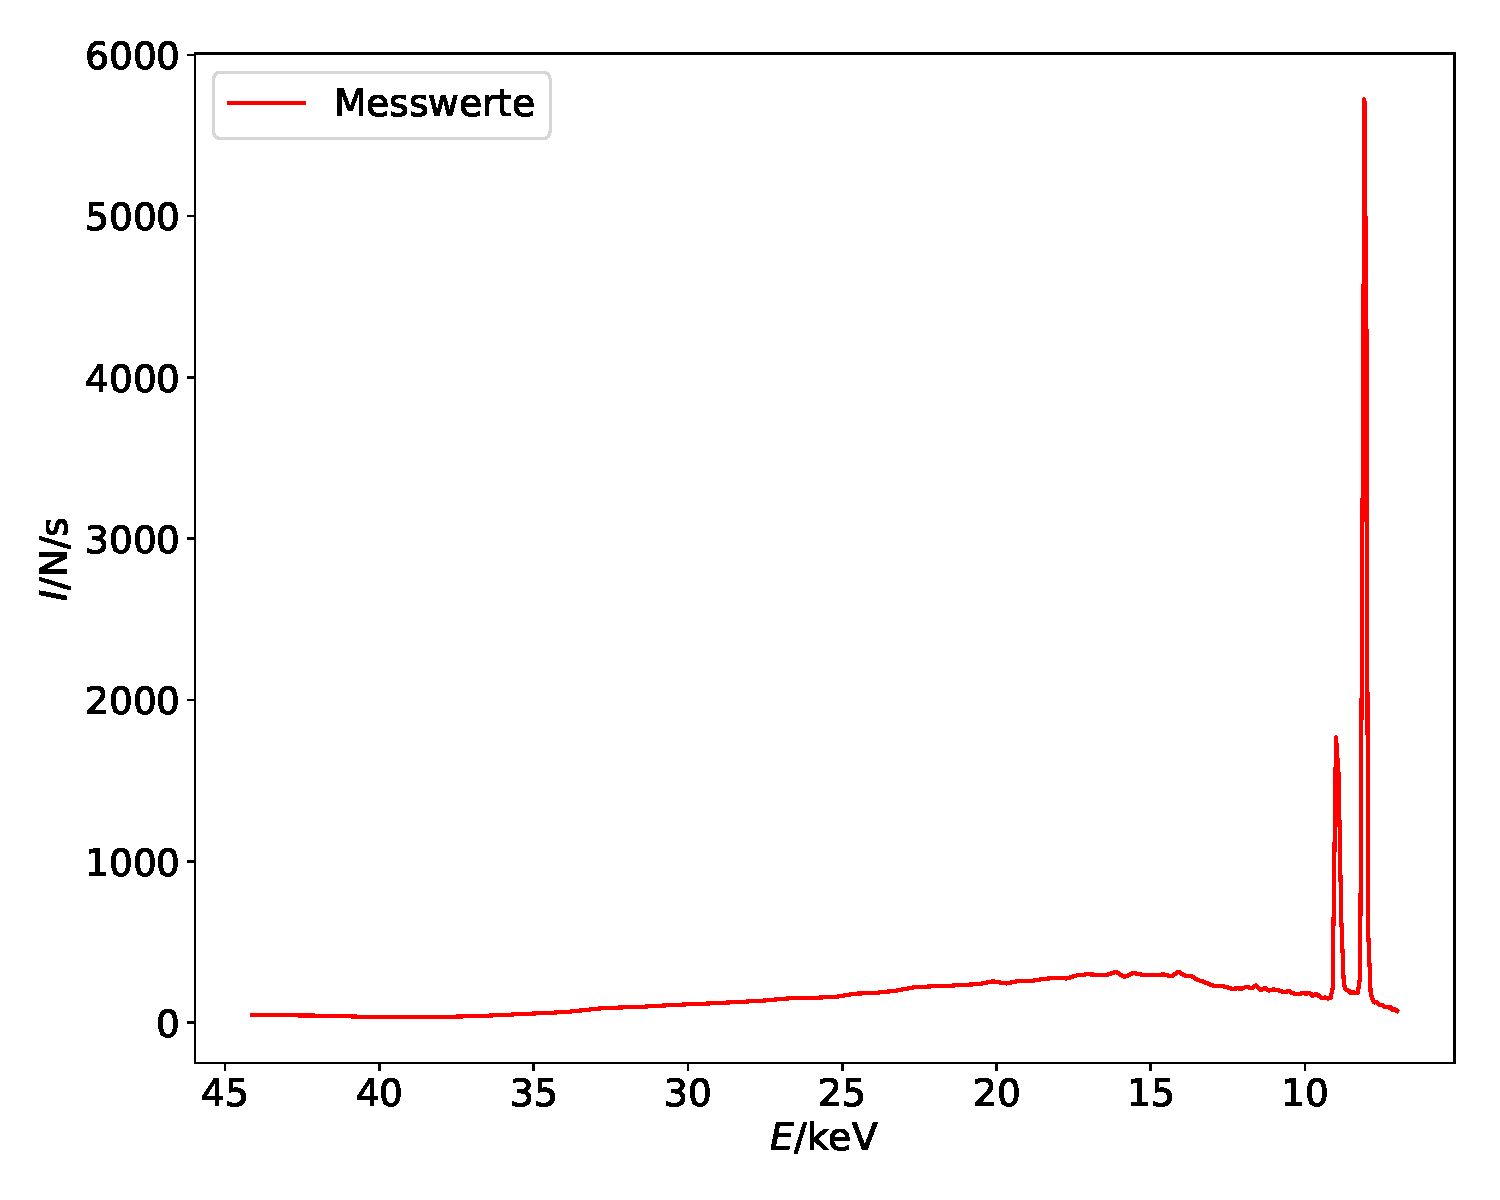
\includegraphics[width=0.4\textwidth]{emission.pdf}
  }
  \hfill
  \subcaptionbox{Messwerte zum Emissionspektrum. \label{tab:1}}[0.8\textwidth]{
    \begin{tabular}{c c c c c c c c}
      \toprule
      $E / \si{\kilo\electronvolt}$ & $I / \si{\per\second}$ & $E / \si{\kilo\electronvolt}$ & $I / \si{\per\second}$ &
      $E / \si{\kilo\electronvolt}$ & $I / \si{\per\second}$ & $E / \si{\kilo\electronvolt}$ & $I / \si{\per\second}$ \\
      \midrule
      44.126 & 47 & 18.457 & 272 & 11.740 & 213 & 8.688 & 207 \\
      42.028 & 44 & 18.084 & 277 & 11.591 & 232 & 8.589 & 199 \\
      40.121 & 35 & 17.726 & 274 & 11.446 & 202 & 8.512 & 185 \\
      38.380 & 34 & 17.382 & 294 & 11.305 & 216 & 8.436 & 187 \\
      36.785 & 41 & 17.051 & 300 & 11.167 & 199 & 8.361 & 186 \\
      35.317 & 54 & 16.733 & 297 & 11.033 & 206 & 8.288 & 186 \\
      33.962 & 66 & 16.427 & 296 & 10.902 & 204 & 8.217 & 285 \\
      32.708 & 91 & 16.132 & 314 & 10.774 & 194 & 8.146 & 2915 \\
      31.543 & 98 & 15.847 & 284 & 10.650 & 190 & 8.077 & 5724 \\
      30.459 & 110 & 15.573 & 308 & 10.528 & 197 & 8.010 & 4243 \\
      29.447 & 118 & 15.308 & 298 & 10.409 & 183 & 7.960 & 584 \\
      28.501 & 127 & 15.052 & 293 & 10.293 & 177 & 7.878 & 187 \\
      27.614 & 136 & 14.805 & 297 & 10.180 & 177 & 7.813 & 144 \\
      26.780 & 150 & 14.566 & 299 & 10.096 & 184 & 7.750 & 125 \\
      25.996 & 154 & 14.334 & 287 & 9.961 & 179 & 7.688 & 131 \\
      25.257 & 159 & 14.110 & 316 & 9.855 & 185 & 7.628 & 115 \\
      24.559 & 180 & 13.893 & 291 & 9.752 & 167 & 7.568 & 109 \\
      23.899 & 185 & 13.683 & 289 & 9.650 & 178 & 7.509 & 109 \\
      23.273 & 198 & 13.480 & 265 & 9.576 & 170 & 7.451 & 103 \\
      22.680 & 219 & 13.282 & 253 & 9.454 & 153 & 7.394 & 95 \\
      22.117 & 225 & 13.090 & 237 & 9.360 & 156 & 7.338 & 97 \\
      21.581 & 228 & 12.904 & 226 & 9.267 & 150 & 7.283 & 94 \\
      21.196 & 233 & 12.723 & 228 & 9.176 & 154 & 7.229 & 95 \\
      20.584 & 239 & 12.548 & 222 & 9.109 & 212 & 7.176 & 80 \\
      20.120 & 256 & 12.377 & 209 & 9.000 & 1769 & 7.124 & 86 \\
      19.676 & 243 & 12.211 & 213 & 8.914 & 1538 & 7.072 & 81 \\
      19.252 & 260 & 12.050 & 211 & 8.830 & 658 & 7.022 & 73 \\
      18.846 & 259 & 11.893 & 224 & 8.748 & 245 & & \\
    \bottomrule
  \end{tabular}
  \hfill
  }
  \caption{Das Emissionspektrum von Kupfer.}
\end{figure}
In Abbildung \ref{fig:2} ist das Emissionspektrum von Kupfer zu sehen. Unser Ausschnitt
des Emissionsspektrum zeigt den Bremsberg von etwa
$\SI{45}{\kilo\electronvolt}$ bis ca. $\SI{9}{\kilo\electronvolt}$. Tatsächlich ist
er dort noch nicht zu Ende, da nur ein Ausschnitt aufgenommen wurde.
Bei $E_\beta = \SI{9}{\kilo\electronvolt}$ die $K_\beta$-Linie und bei $E_\alpha = \SI{8.077}{\kilo\electronvolt}$
die $K_\alpha$-Linie. Bei einem Grenzwinkel von 10° ergibt sich nach \eqref{eq:3} mit
der Beziehung
\begin{equation}
  E = c \cdot 1/\lambda
  \label{eqn:1}
\end{equation}
die Gleichung
\begin{equation}
  E = c \cdot \frac{h}{2 \, d \, \symup{sin}(\theta)} \, .
  \label{eqn:2}
\end{equation}
Mit $d = \SI{201.4}{\pico\meter}$ ergibt sich die maximale Energie zu $E_{\symup{Grenz}} = \SI{35.32}{\kilo\electronvolt}$.
Für die Abschirmkonstanten $\sigma_K$ und $\sigma_L$ wird ausgenutzt, dass $E_\beta$ ungefähr der
Bindungsenergie $E_k$ aus \eqref{eqn:3} entspricht. Damit ergeben sich folgenden Formeln
\begin{align}
    \sigma_K &= z_{Cu} - \sqrt{\frac{E_\beta}{E_\symup{Ryd}}} \\
    \sigma_L &= z_{Cu} - \sqrt{\frac{4(E_\beta - E_\alpha)}{E_\symup{Ryd}}} \, .
\end{align}
Für die oben angegebenen Energien ergeben sich für die Abschirmkonstanten
\begin{align*}
    \sigma_K &= \num{3.28} \\
    \sigma_L &= \num{12.52} \, .
\end{align*}
\\
Die Halbwertsbreiten lassen sich aus Tabelle \ref{tab:2} ablesen. Die Untergrundstrahlung
wird für $K_\beta$ bei $\SI{9.176}{\kilo\electronvolt}$ und bei $\SI{8.688}{\kilo\electronvolt}$
und für $K_\alpha$ bei $\SI{8.288}{\kilo\electronvolt}$ und bei $\SI{7.878}{\kilo\electronvolt}$.
Die Breiten der Linien betragen $\SI{0.488}{\kilo\electronvolt}$ bzw. $\SI{0.410}{\kilo\electronvolt}$.
Daraus ergeben sich für die Halbwertsbreiten $\Delta_{1/2}$
\begin{align*}
  \Delta_{1/2} K_\beta &= \SI{244}{\electronvolt} \\
  \Delta_{1/2} K_\alpha &= \SI{205}{\electronvolt} \, .
\end{align*}

\subsection{Absorptionsspektren von leichten und schweren Elementen.}
\begin{figure}
  \centering
  \subcaptionbox{Graphische Darstellung der Messwerte. \label{sub:3}}[0.7\textwidth]{
  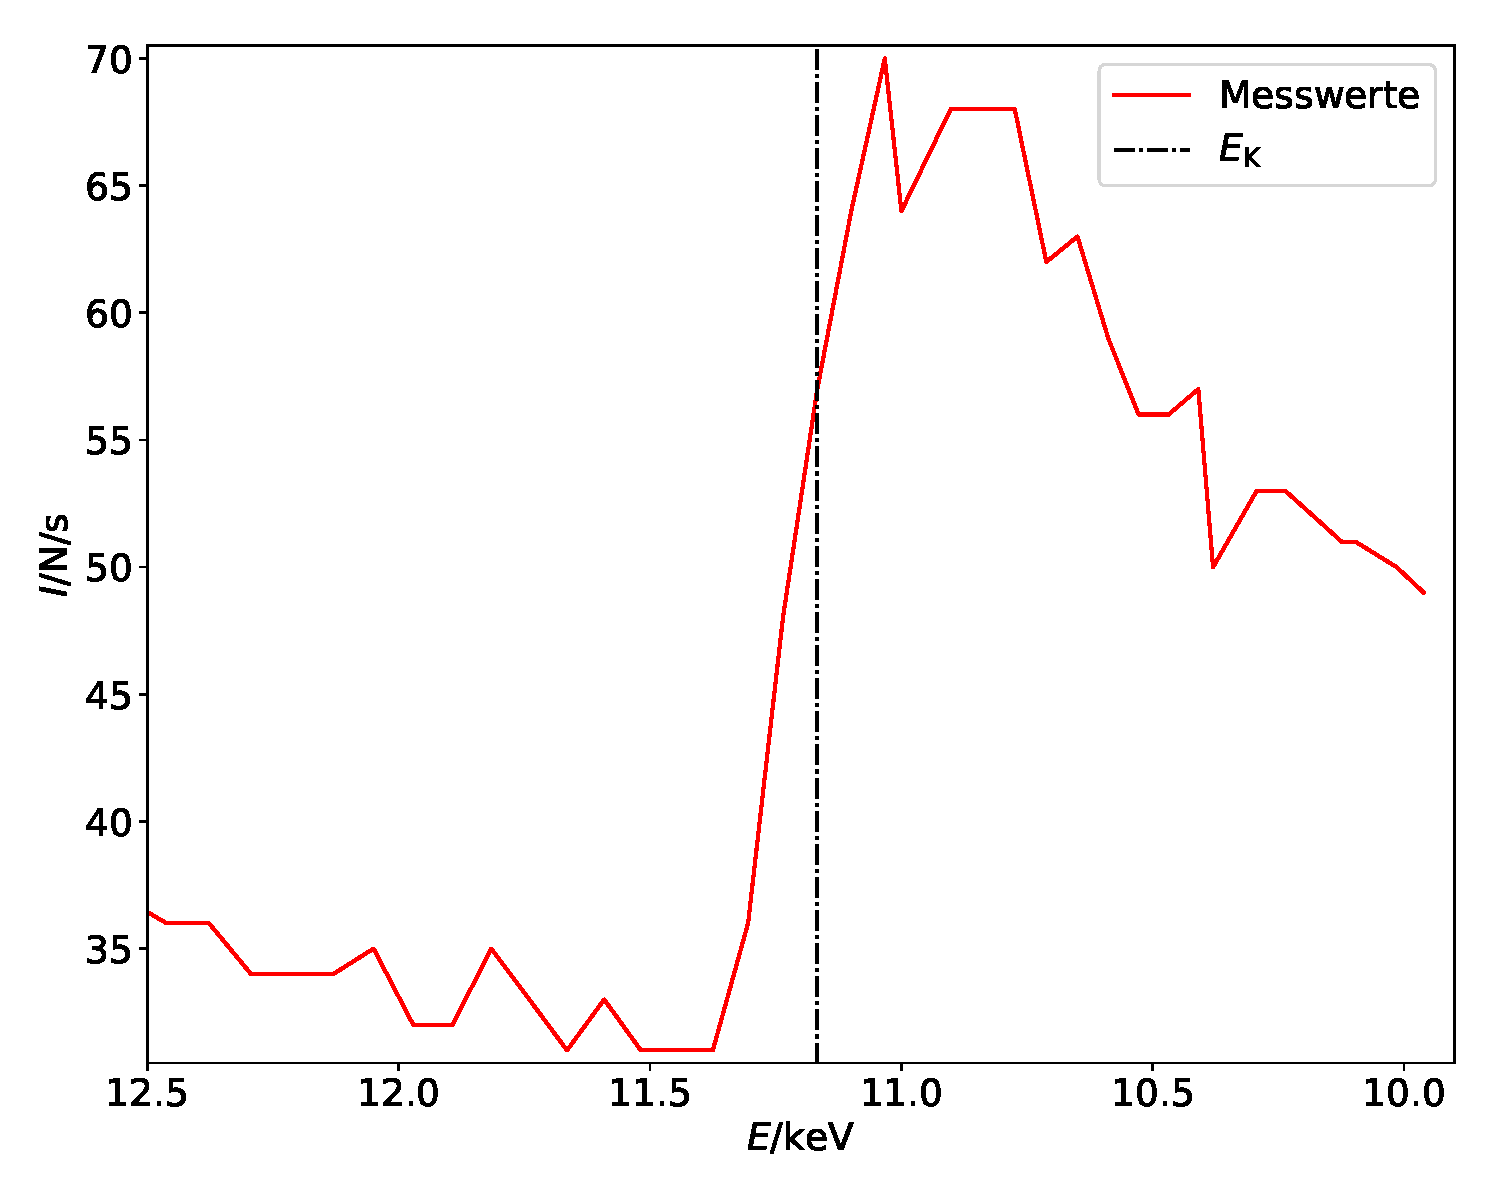
\includegraphics[width=0.7\textwidth]{germanium.pdf}
  }
  \hfill
  \subcaptionbox{Messwerte. \label{tab:2}}[0.29\textwidth]{
  \begin{tabular}{c c}
    \toprule
    $E / \si{\kilo\electronvolt}$ & $I / \si{\per\second}$ \\
    \midrule
    12.7 & 40 \\
    12.6 & 37 \\
    12.5 & 37 \\
    12.5 & 36 \\
    12.4 & 36 \\
    12.3 & 34 \\
    12.2 & 34 \\
    12.1 & 34 \\
    12.0 & 35 \\
    12.0 & 32 \\
    11.9 & 32 \\
    11.8 & 35 \\
    11.7 & 33 \\
    11.7 & 31 \\
    11.6 & 33 \\
    11.5 & 31 \\
    11.4 & 31 \\
    11.4 & 31 \\
    11.3 & 36 \\
    11.2 & 48 \\
    11.2 & 57 \\
    11.1 & 64 \\
    11.0 & 70 \\
    11.0 & 64 \\
    10.9 & 68 \\
    10.8 & 68 \\
    10.8 & 68 \\
    10.7 & 62 \\
    10.6 & 63 \\
    10.6 & 59 \\
    10.5 & 56 \\
    10.5 & 56 \\
    10.4 & 57 \\
    10.4 & 50 \\
    10.3 & 53 \\
    10.2 & 53 \\
    10.2 & 52 \\
    10.1 & 51 \\
    10.1 & 51 \\
    10.0 & 50 \\
    10.0 & 49 \\
    \bottomrule
  \end{tabular}
  }
  \caption{Absorptionsspektrum von Germanium.}
  \label{fig:3}
\end{figure}
\begin{figure}
  \centering
  \subcaptionbox{Graphische Darstellung der Messwerte. \label{sub:4}}[0.7\textwidth]{
  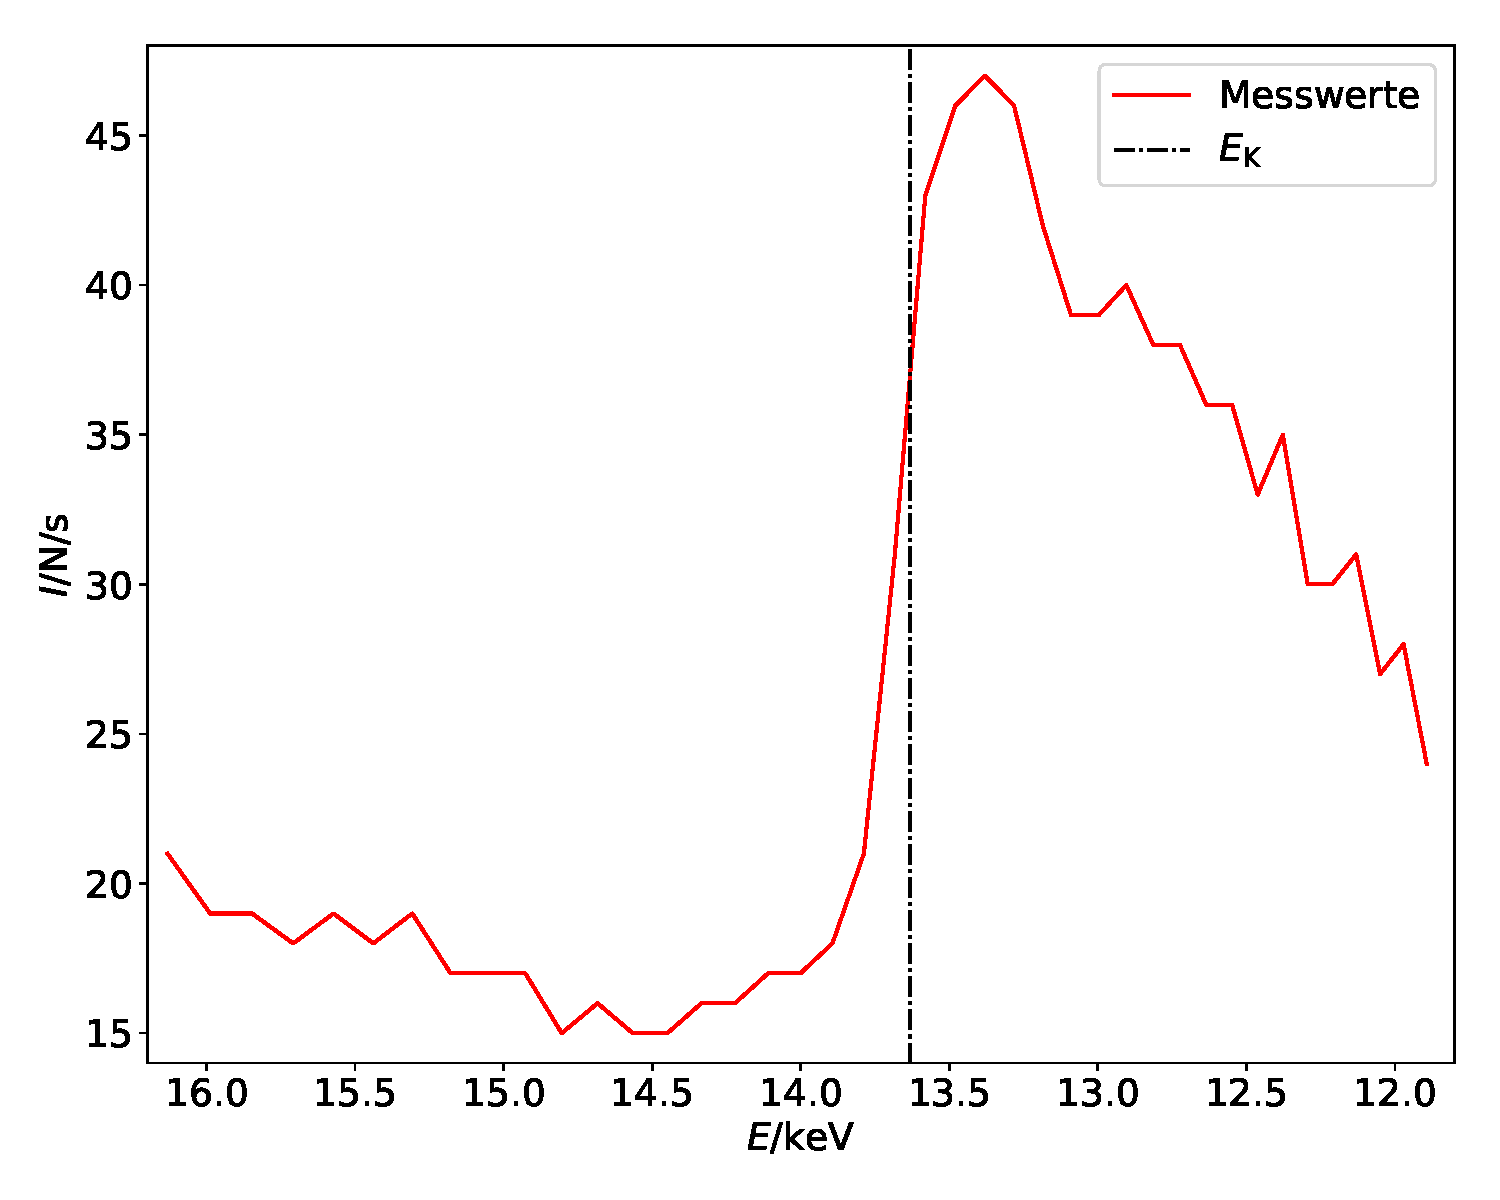
\includegraphics[width=0.7\textwidth]{brom.pdf}
  }
  \hfill
  \subcaptionbox{Messwerte. \label{tab:3}}[0.29\textwidth]{
  \begin{tabular}{c c}
    \toprule
    $E / \si{\kilo\electronvolt}$ & $I / \si{\per\second}$ \\
    \midrule
    16.1 & 21 \\
    16.0 & 19 \\
    15.8 & 19 \\
    15.7 & 18 \\
    15.6 & 19 \\
    15.4 & 18 \\
    15.3 & 19 \\
    15.2 & 17 \\
    15.1 & 17 \\
    14.9 & 17 \\
    14.8 & 15 \\
    14.7 & 16 \\
    14.6 & 15 \\
    14.4 & 15 \\
    14.3 & 16 \\
    14.2 & 16 \\
    14.1 & 17 \\
    14.0 & 17 \\
    13.9 & 18 \\
    13.8 & 21 \\
    13.7 & 31 \\
    13.6 & 43 \\
    13.5 & 46 \\
    13.4 & 47 \\
    13.3 & 46 \\
    13.2 & 42 \\
    13.1 & 39 \\
    13.0 & 39 \\
    12.9 & 40 \\
    12.8 & 38 \\
    12.7 & 38 \\
    12.6 & 36 \\
    12.5 & 36 \\
    12.5 & 33 \\
    12.4 & 35 \\
    12.3 & 30 \\
    12.2 & 30 \\
    12.1 & 31 \\
    12.0 & 27 \\
    12.0 & 28 \\
    11.9 & 24 \\
    \bottomrule
  \end{tabular}
  }
  \caption{Absorptionsspektrum von Brom.}
  \label{fig:4}
\end{figure}

\begin{figure}
  \centering
  \subcaptionbox{Graphische Darstellung der Messwerte. \label{sub:5}}[0.7\textwidth]{
  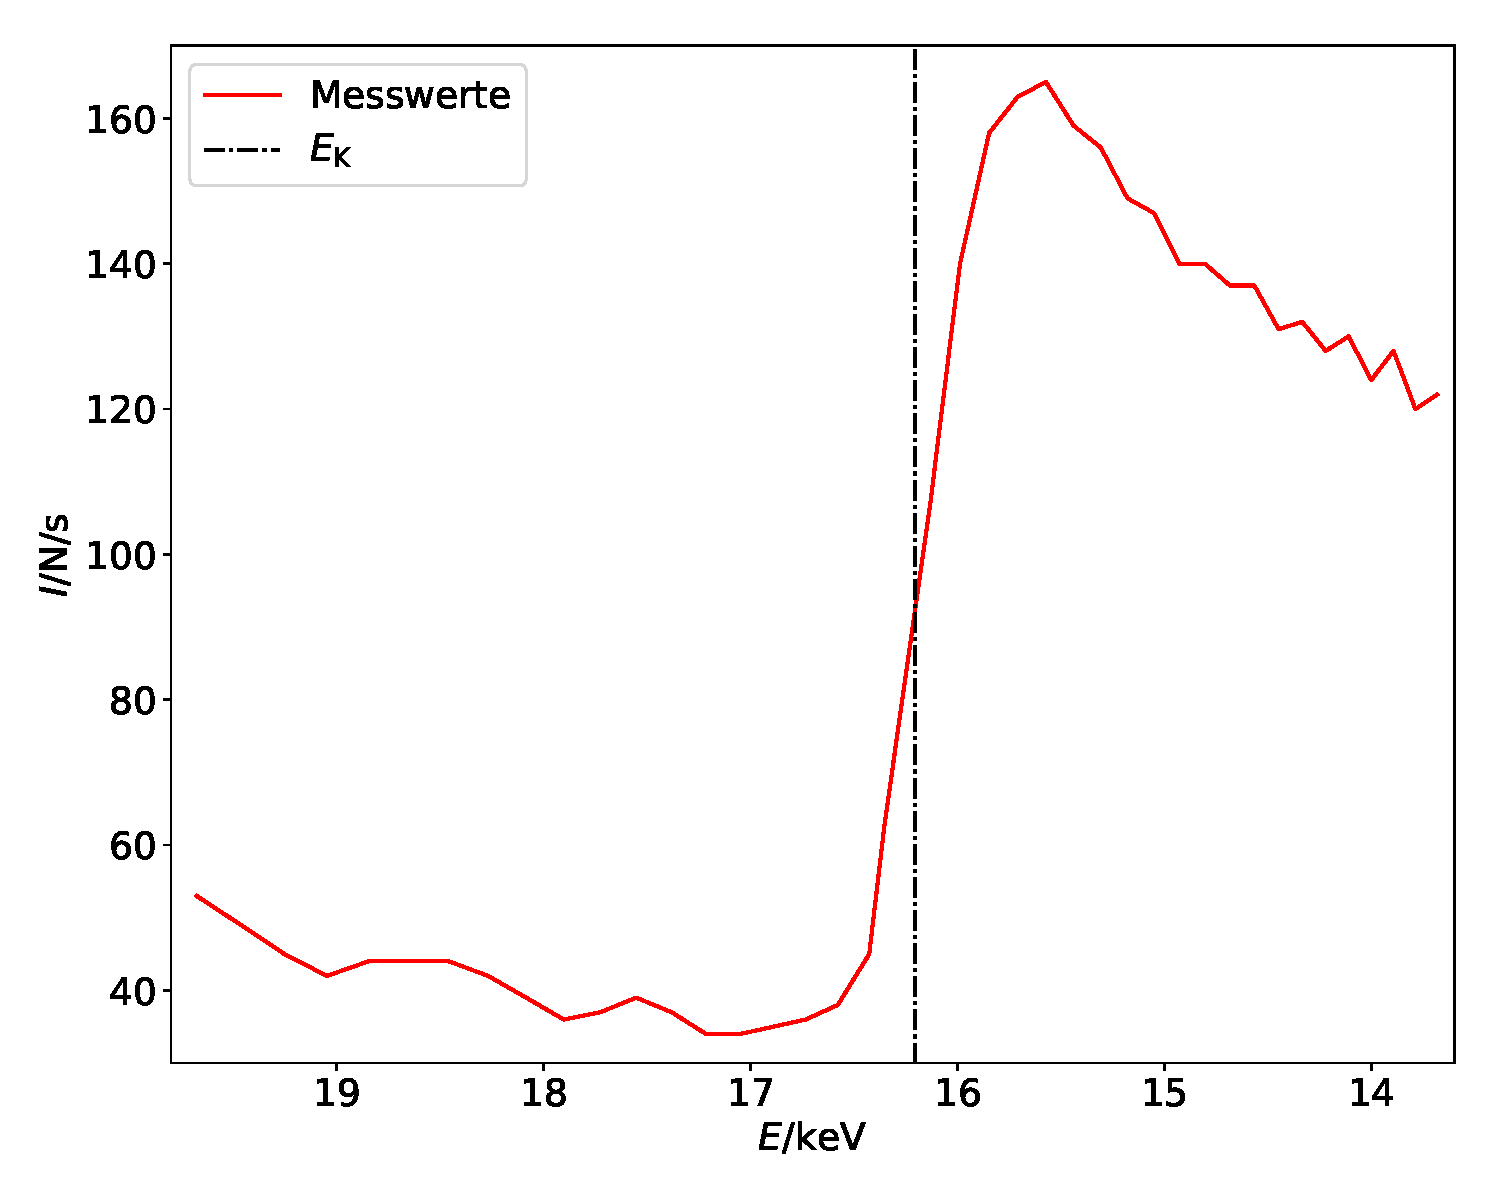
\includegraphics[width=0.7\textwidth]{strontium.pdf}
  }
  \hfill
  \subcaptionbox{Messwerte. \label{tab:4}}[0.29\textwidth]{
  \begin{tabular}{c c}
    \toprule
    $E / \si{\kilo\electronvolt}$ & $I / \si{\per\second}$ \\
    \midrule
    19.7 & 53 \\
    19.5 & 49 \\
    19.3 & 45 \\
    19.0 & 42 \\
    18.8 & 44 \\
    18.6 & 44 \\
    18.5 & 44 \\
    18.3 & 42 \\
    18.1 & 39 \\
    17.9 & 36 \\
    17.7 & 37 \\
    17.6 & 39 \\
    17.4 & 37 \\
    17.2 & 34 \\
    17.1 & 34 \\
    16.9 & 35 \\
    16.7 & 36 \\
    16.6 & 38 \\
    16.4 & 45 \\
    16.4 & 63 \\
    16.1 & 107 \\
    16.0 & 140 \\
    15.8 & 158 \\
    15.7 & 163 \\
    15.6 & 165 \\
    15.4 & 159 \\
    15.3 & 156 \\
    15.2 & 149 \\
    15.1 & 147 \\
    14.9 & 140 \\
    14.8 & 140 \\
    14.7 & 137 \\
    14.6 & 137 \\
    14.4 & 131 \\
    14.3 & 132 \\
    14.2 & 128 \\
    14.1 & 130 \\
    14.0 & 124 \\
    13.9 & 128 \\
    13.8 & 120 \\
    13.7 & 122 \\
    \bottomrule
  \end{tabular}
  }
  \caption{Absorptionsspektrum von Strontium.}
  \label{fig:5}
\end{figure}

\begin{figure}
  \centering
  \subcaptionbox{Graphische Darstellung der Messwerte. \label{sub:6}}[0.7\textwidth]{
  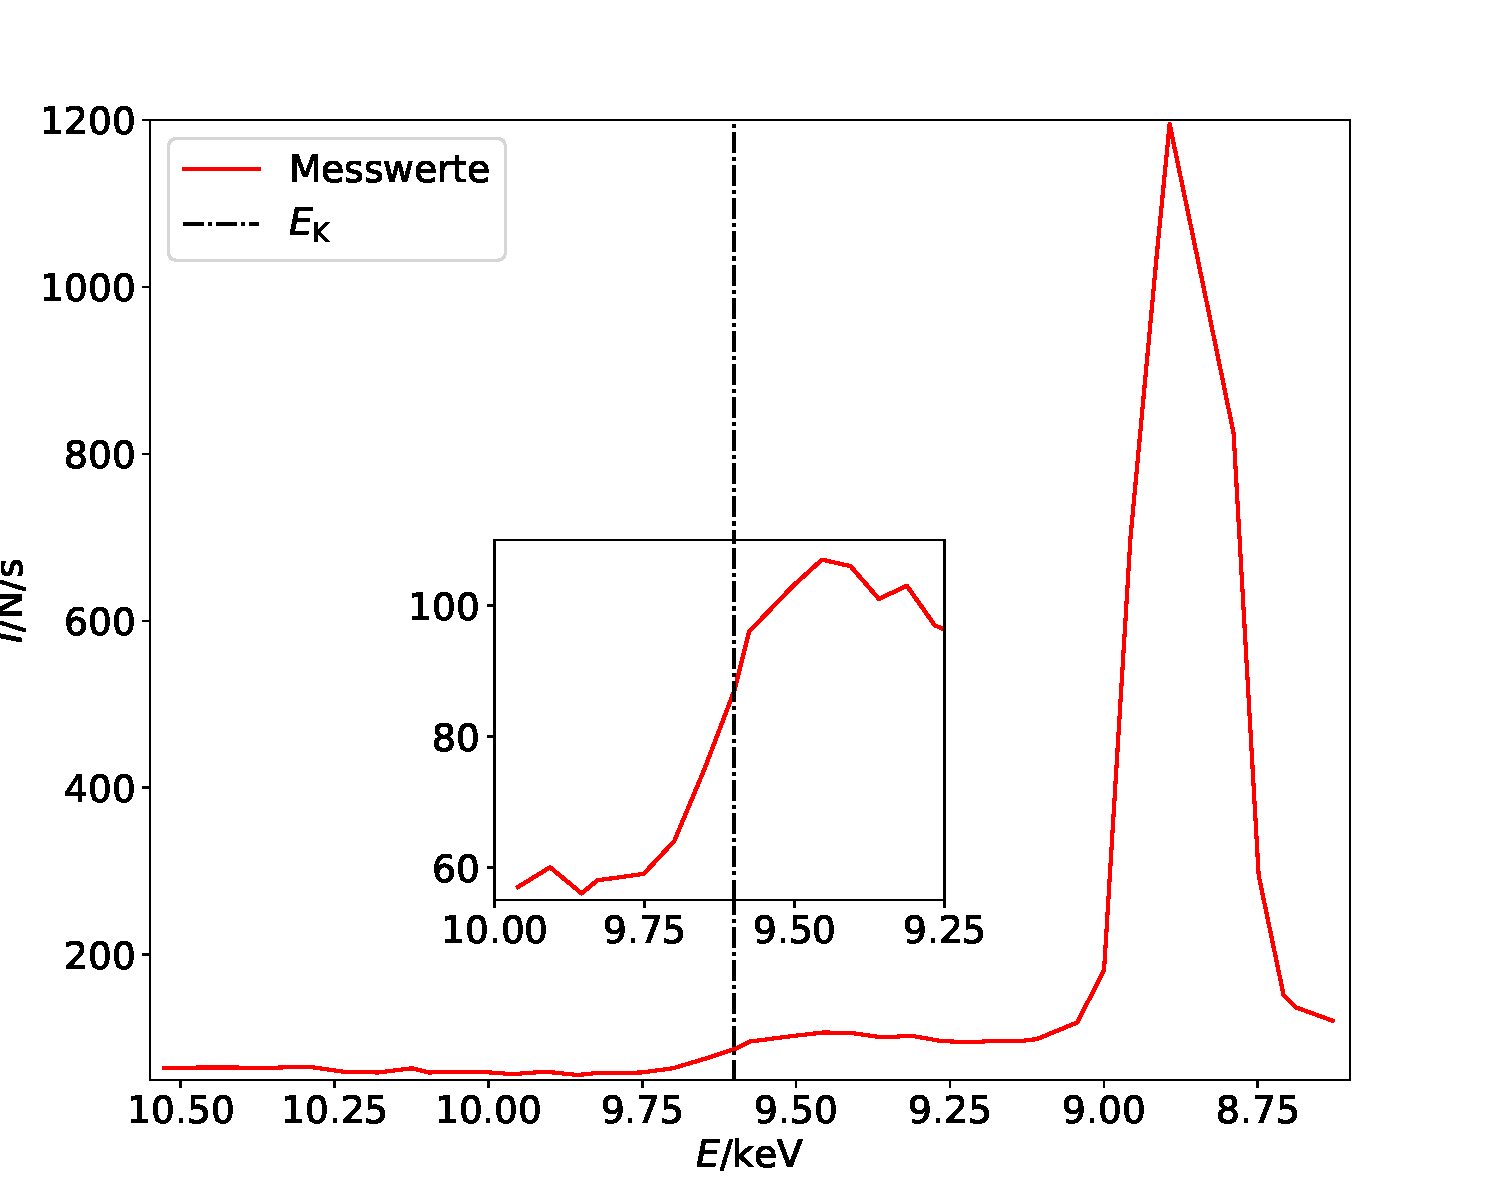
\includegraphics[width=0.7\textwidth]{zink.pdf}
  }
  \hfill
  \subcaptionbox{Messwerte. \label{tab:5}}[0.29\textwidth]{
  \begin{tabular}{c c}
    \toprule
    $E / \si{\kilo\electronvolt}$ & $I / \si{\per\second}$ \\
    \midrule
    10.5 & 64 \\
    10.5 & 65 \\
    10.4 & 65 \\
    10.4 & 64 \\
    10.3 & 66 \\
    10.2 & 60 \\
    10.2 & 59 \\
    10.1 & 64 \\
    10.1 & 59 \\
    10.0 & 60 \\
    10.0 & 57 \\
    9.9 & 60 \\
    9.9 & 56 \\
    9.8 & 58 \\
    9.8 & 59 \\
    9.7 & 64 \\
    9.7 & 75 \\
    9.6 & 87 \\
    9.6 & 96 \\
    9.5 & 103 \\
    9.5 & 107 \\
    9.4 & 106 \\
    9.4 & 101 \\
    9.3 & 103 \\
    9.3 & 97 \\
    9.2 & 95 \\
    9.2 & 97 \\
    9.1 & 97 \\
    9.1 & 99 \\
    9.0 & 119 \\
    9.0 & 182 \\
    9.0 & 700 \\
    8.9 & 1037 \\
    8.9 & 1195 \\
    8.8 & 973 \\
    8.8 & 825 \\
    8.7 & 295 \\
    8.7 & 152 \\
    8.7 & 137 \\
    8.6 & 121 \\
    \bottomrule
  \end{tabular}
  }
  \caption{Absorptionsspektrum von Zink.}
  \label{fig:6}
\end{figure}

\begin{figure}
  \centering
  \subcaptionbox{Graphische Darstellung der Messwerte. \label{sub:7}}[0.7\textwidth]{
  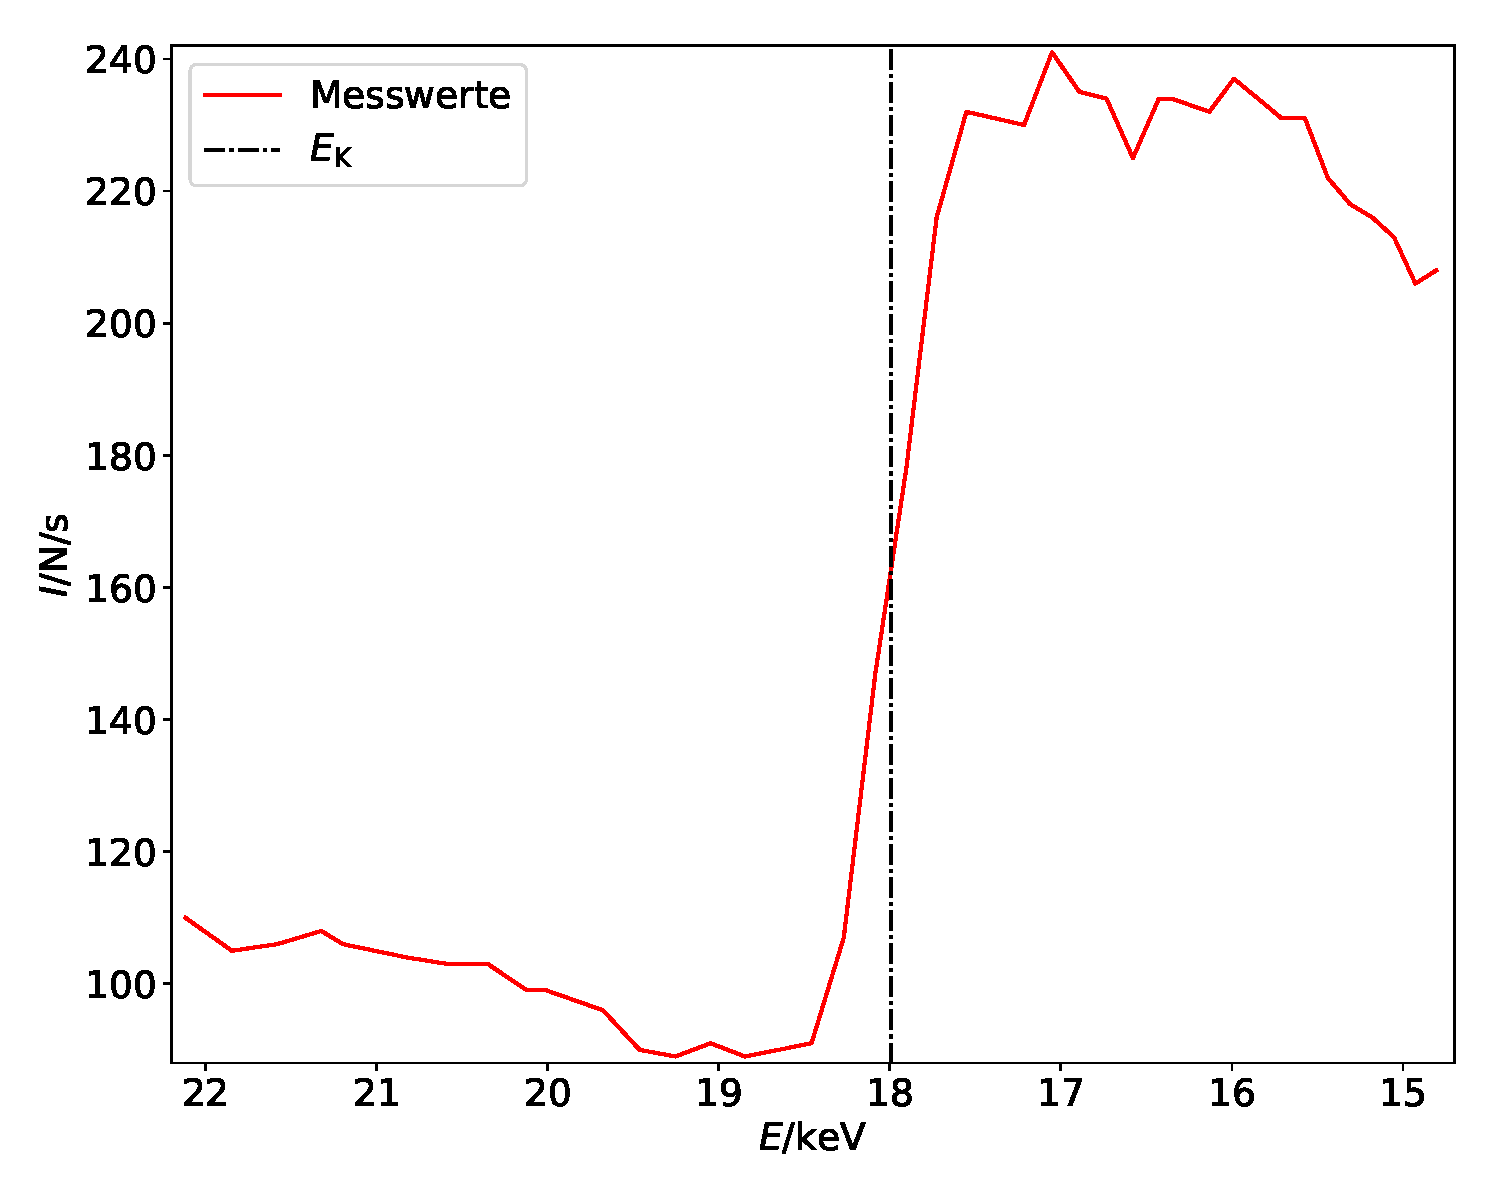
\includegraphics[width=0.7\textwidth]{zirkonium.pdf}
  }
  \hfill
  \subcaptionbox{Messwerte. \label{tab:6}}[0.29\textwidth]{
  \begin{tabular}{c c}
    \toprule
    $E / \si{\kilo\electronvolt}$ & $I / \si{\per\second}$ \\
    \midrule
    22.1 & 110 \\
    21.8 & 105 \\
    21.6 & 106 \\
    21.3 & 108 \\
    21.2 & 106 \\
    20.8 & 104 \\
    20.6 & 103 \\
    20.3 & 103 \\
    20.1 & 99 \\
    20.0 & 99 \\
    19.7 & 96 \\
    19.5 & 90 \\
    19.3 & 89 \\
    19.0 & 91 \\
    18.8 & 89 \\
    18.6 & 90 \\
    18.5 & 91 \\
    18.3 & 107 \\
    18.1 & 147 \\
    17.9 & 178 \\
    17.7 & 216 \\
    17.6 & 232 \\
    17.4 & 231 \\
    17.2 & 230 \\
    17.1 & 241 \\
    16.9 & 235 \\
    16.7 & 234 \\
    16.6 & 225 \\
    16.4 & 234 \\
    16.4 & 234 \\
    16.1 & 232 \\
    16.0 & 237 \\
    15.8 & 234 \\
    15.7 & 231 \\
    15.6 & 231 \\
    15.4 & 222 \\
    15.3 & 218 \\
    15.2 & 216 \\
    15.1 & 213 \\
    14.9 & 206 \\
    14.8 & 208 \\
    \bottomrule
  \end{tabular}
  }
  \caption{Absorptionsspektrum von Zirkonium.}
  \label{fig:7}
\end{figure}
Für die verschiedenen Materialien ergeben sich die Absorptionsenergien aus den Plots \ref{sub:3} bis
\ref{sub:7} und
aus der Formel
\begin{equation}
  \sigma_K = z - \sqrt{\frac{E_k}{E_\symup{Ryd}} - \frac{\alpha^2 \, z^4}{4}}
  \label{eqn:4}
\end{equation}
die Abschirmkonstanten.

\begin{table}
  \centering
  \caption{K-Kanten Energien für die verschiedenen Materialien und die daraus resultierenden
  Abschirmkonstanten $\sigma_K$.}
  \label{tab:7}
  \begin{tabular}{c c c}
    \toprule
    & $E_K / \si{\kilo\electronvolt}$ & $\sigma_K$ \\
    \midrule
    Germanium & 11.17 & 3.59 \\
    Strontium & 16.20 & 3.89 \\
    Brom & 13.63 & 3.66 \\
    Zink & 9.60 & 3.63 \\
    Zirkonium & 17.99 & 4.10 \\
    \bottomrule
  \end{tabular}
\end{table}
Nach dem Moseleyschen Gesetz ist $\sqrt{E_k} \propto z$. In Abbildung \ref{fig:8}
ist dieser Zusammenhang graphisch dargestellt. Die Steigung zum Quadrat sollte laut
\eqref{eqn:3} genau der Rydbergenergie entsprechen. Es ergibt sich $m^2 = \SI{13.05(31)}{\electronvolt}$.
\begin{figure}
  \centering
  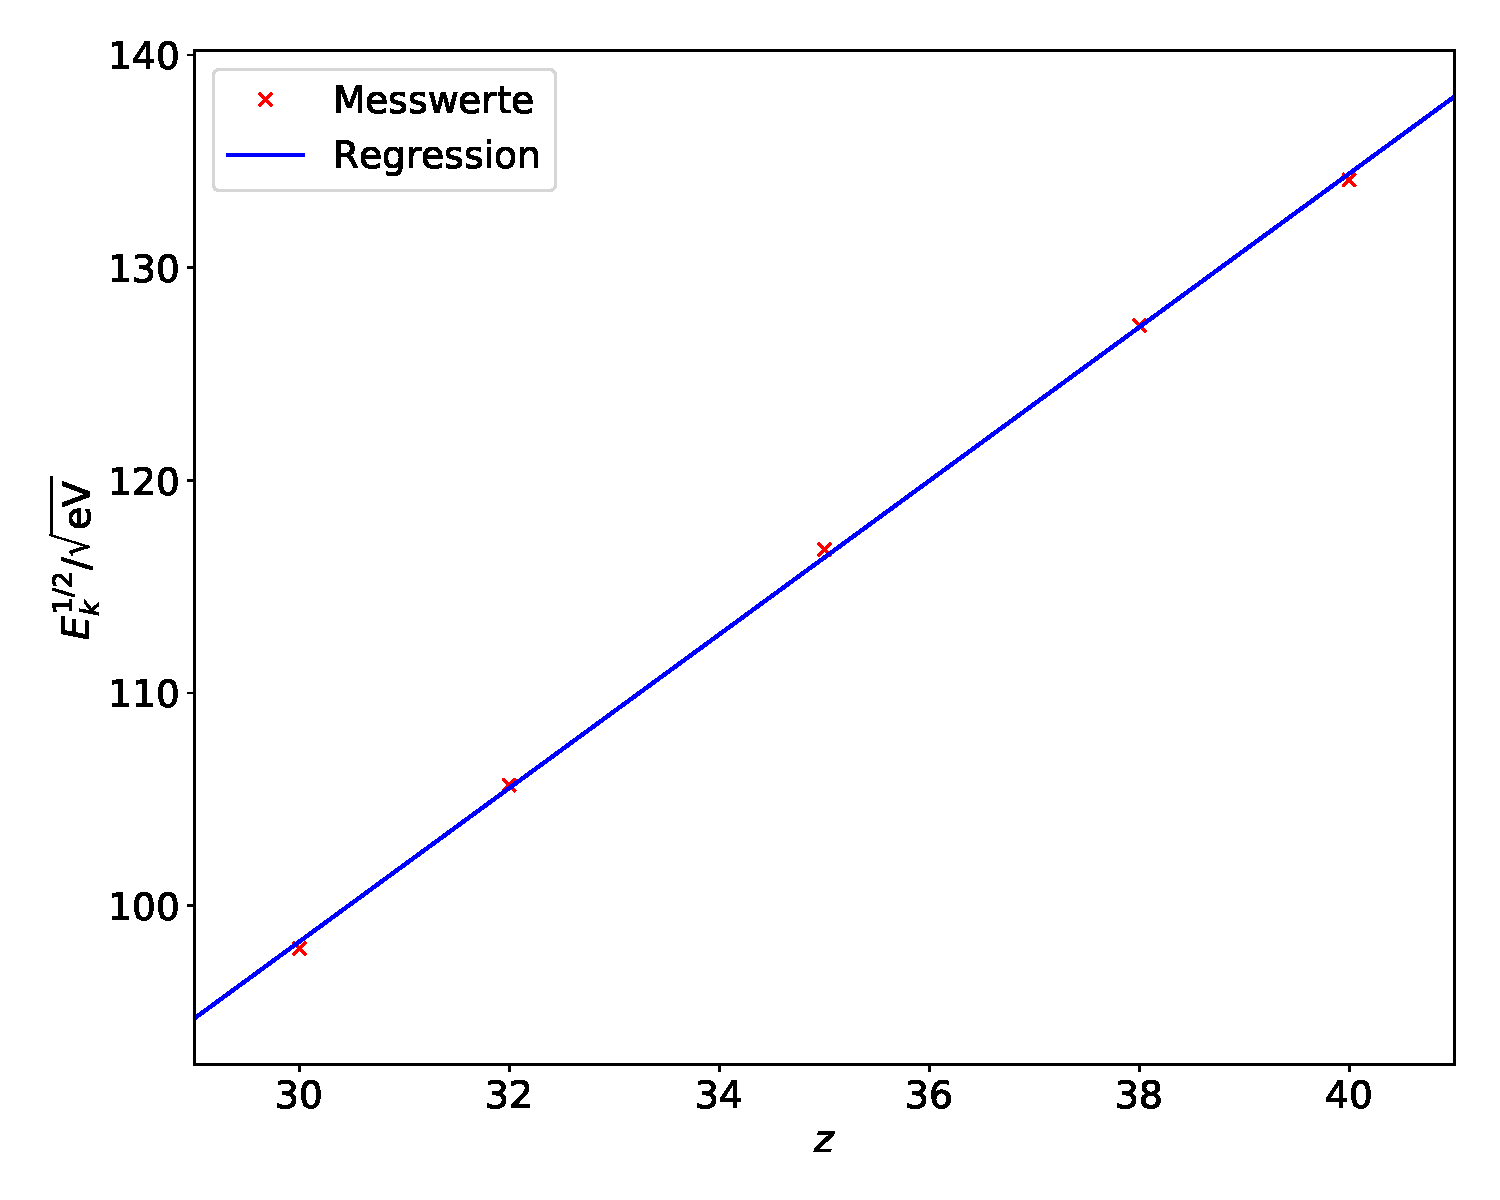
\includegraphics[scale=0.3]{moseley.pdf}
  \caption{Graphische Darstellung des Moseleyschen Gesetzes mit dem oben berechneten
  Energien der K-Kanten mit linearer Regression.}
  \label{fig:8}
\end{figure}

In Abbildung \ref{fig:9} befindet sich das Absorptionsspektrum von Wismut.
\begin{figure}
  \centering
  \subcaptionbox{Graphische Darstellung der Messwerte. \label{sub:9}}[0.7\textwidth]{
  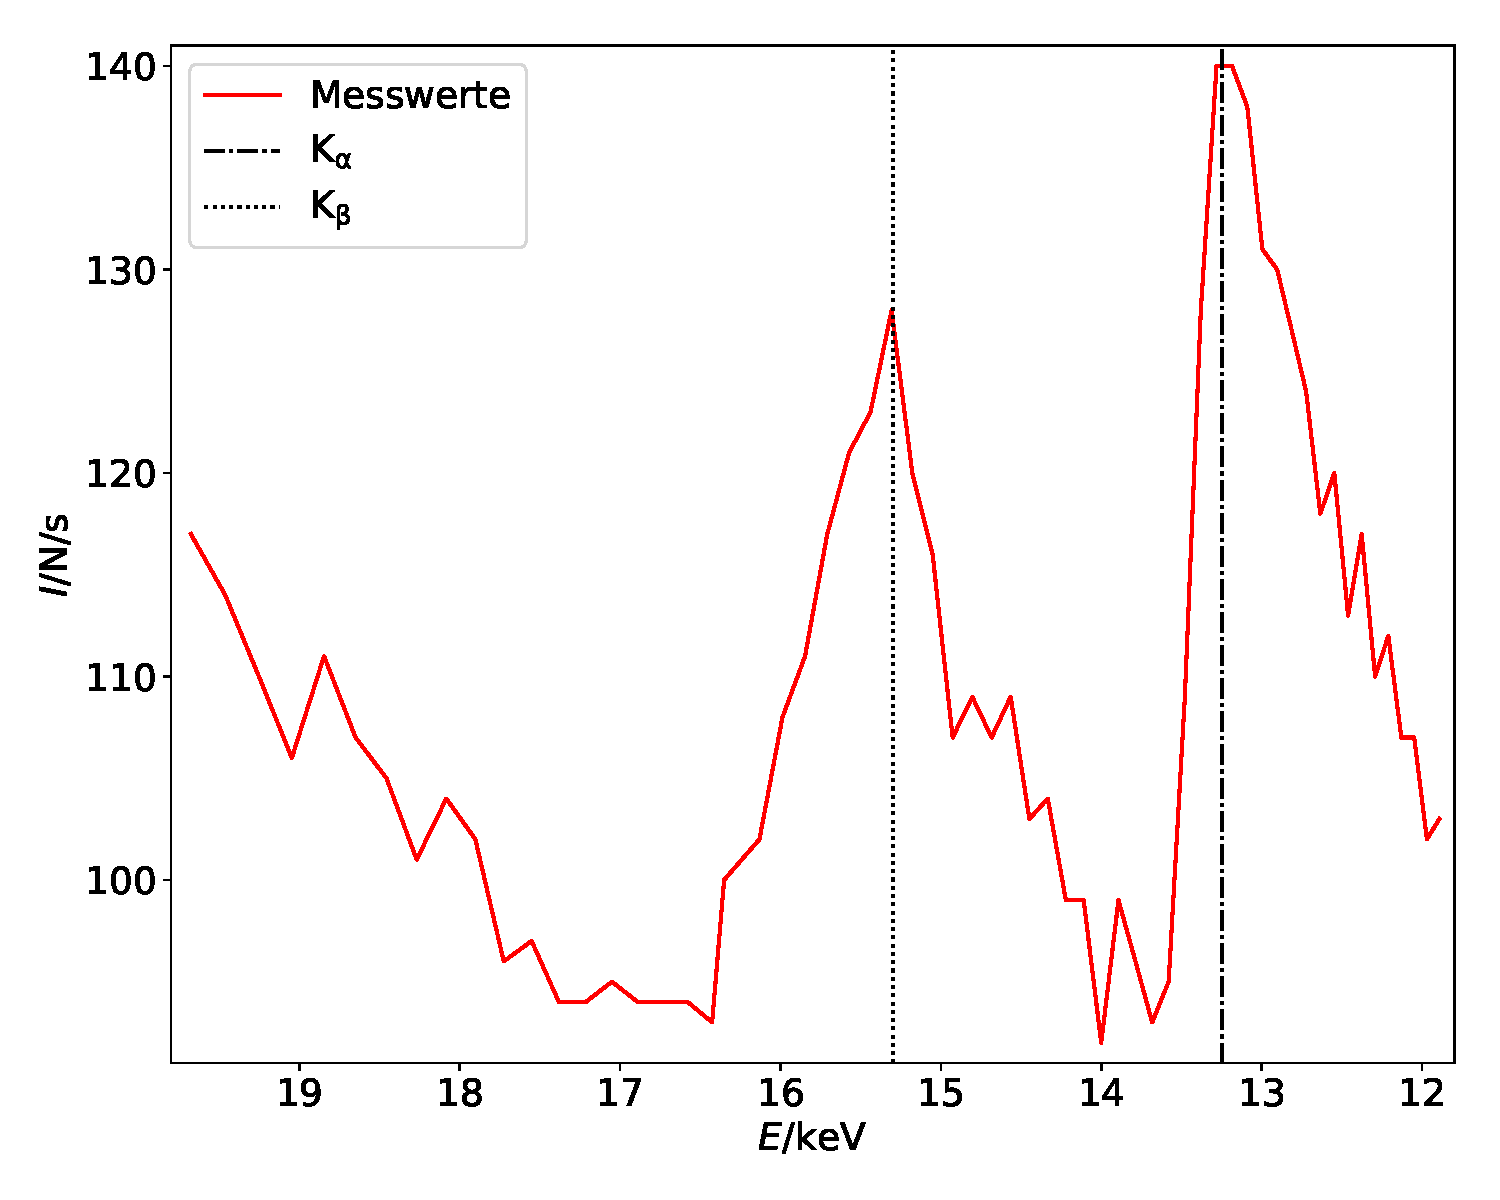
\includegraphics[width=0.7\textwidth]{wismut.pdf}
  }
  \hfill
  \subcaptionbox{Messwerte. \label{tab:9}}[0.29\textwidth]{
  \begin{tabular}{c c c c}
    \toprule
    $E / \si{\kilo\electronvolt}$ & $I / \si{\per\second}$ & $E / \si{\kilo\electronvolt}$ & $I / \si{\per\second}$ \\
    \midrule
    19.7 & 117 & 14.7 & 107 \\
    19.5 & 114 & 14.6 & 109 \\
    19.3 & 110 & 14.4 & 103 \\
    19.0 & 106 & 14.3 & 104 \\
    18.8 & 111 & 14.2 & 99 \\
    18.6 & 107 & 14.1 & 99 \\
    18.5 & 105 & 14.0 & 92 \\
    18.3 & 101 & 13.9 & 99 \\
    18.1 & 104 & 13.8 & 96 \\
    17.9 & 102 & 13.7 & 93 \\
    17.7 & 96 & 13.6 & 95 \\
    17.6 & 97 & 13.5 & 109 \\
    17.4 & 94 & 13.4 & 128 \\
    17.2 & 94 & 13.3 & 140 \\
    17.1 & 95 & 13.2 & 140 \\
    16.9 & 94 & 13.1 & 138 \\
    16.7 & 94 & 13.0 & 131 \\
    16.6 & 94 & 12.9 & 130 \\
    16.4 & 93 & 12.8 & 127 \\
    16.4 & 100 & 12.7 & 124 \\
    16.1 & 102 & 12.6 & 118 \\
    16.0 & 108 & 12.5 & 120 \\
    15.8 & 111 & 12.5 & 113 \\
    15.7 & 117 & 12.4 & 117 \\
    15.6 & 121 & 12.3 & 110 \\
    15.4 & 123 & 12.2 & 112 \\
    15.3 & 128 & 12.1 & 107 \\
    15.2 & 120 & 12.0 & 107 \\
    15.1 & 116 & 12.0 & 102 \\
    14.9 & 107 & 11.9 & 103 \\
    14.8 & 109 & & \\
    \bottomrule
  \end{tabular}
  }
  \caption{Absorptionsspektrum von Wismut.}
  \label{fig:9}
\end{figure}
Für die Abschirmkonstante ergibt sich mit
\begin{equation}
  \sigma_L = z - \left(\frac{4}{\alpha}\sqrt{\frac{\Delta E_L}{E_\symup{Ryd}}} - \frac{5\Delta E_L}{E_\symup{Ryd}} \right)^{1/2}
  \left(1 + \frac{19}{32} \, \alpha^2 \frac{\Delta E_L}{E_\symup{Ryd}} \right)^{1/2}
  \label{eqn:5}
\end{equation}
der Wert $\sigma_L = \num{5.51}$. Dabei ist $\Delta E_L$ die Differenz zwischen den Energien
der $L_{II}$ - und der $L_{III}$ - Kante.


\section{Diskussion}
\newpage
\nocite{*}
\printbibliography
